% Supplementary Information for the Scientific Reports manuscript. Build: pdflatex neurosafe_scirep_SI.tex
\documentclass[11pt,a4paper]{article}
\usepackage[utf8]{inputenc}
\usepackage[T1]{fontenc}
\usepackage{lmodern}
\usepackage[margin=2.5cm]{geometry}
\usepackage{amsmath,amssymb,booktabs,graphicx,url}
\usepackage[hidelinks]{hyperref}
\renewcommand{\thetable}{S\arabic{table}}
\renewcommand{\thefigure}{S\arabic{figure}}
\renewcommand{\figurename}{Supplementary Figure}
\renewcommand{\tablename}{Supplementary Table}
\setlength{\parskip}{3pt}
\title{\large\bfseries Supplementary Information for\\[3pt]
Context-conditional feasibility improves safe sequential decisions only as far as the observed context reveals harm}
\author{Mahmudul Hasan Joy and Syed Mehedi Hussain}
\date{}
\begin{document}
\maketitle

\section*{Supplementary Note 1: Reproducing every result}
{\sloppy Use Python 3.11.9 with the package versions in \texttt{requirements-lock.txt}. Install
\texttt{safeopt==0.16} and copy \texttt{patched\_safeopt/*.py} over the installed package, as its README
describes; the patch consists of 15 compatibility lines (\texttt{collections}$\to$\texttt{collections.abc}
for Python $\ge$3.10, and \texttt{np.float}/\texttt{np.bool}$\to$\texttt{float}/\texttt{bool} for NumPy
$\ge$1.24) and no other change, which \texttt{experiments/diff\_safeopt.py} verifies. Run from the
repository root, in order:\par}
{\footnotesize
\begin{verbatim}
python experiments/run_v3.py frontier --domain scm --seeds 100:150 \
    --agents "NeuroSafe-Ctx,Chance,SafeGP,Conservative"     # also lending, ihdp
python experiments/regen_domain.py scm       # tuning seeds, defaults, ablations; also ihdp
python experiments/regen_lending.py          # the same for lending
python experiments/run_safeopt_ref.py --domain scm           # also lending, ihdp
python experiments/run_ablation2.py
python experiments/swap_ihdp_ablation.py
python experiments/analyze_v3.py scm         # each domain
python experiments/channel_ceiling.py
python experiments/verify_theorem.py
python experiments/verify_floor.py
python experiments/figures_v3.py
python experiments/make_fig_domains.py
python experiments/make_tables_v3.py
python experiments/make_posthoc_betacell.py
python experiments/mimic_audit.py            # requires credentialed MIMIC-IV access
python experiments/make_mimic_tables.py
\end{verbatim}}
Tuning uses seeds 0--9 and evaluation seeds 100--149; the two sets do not overlap. The lending
environment's fitted default model is fingerprinted by \texttt{experiments/lending\_fingerprint.py}
(prediction hash \texttt{ebe8497b2903d8e0} in the reported environment).

\section*{Supplementary Note 2: Cross-environment comparison}
Every result was regenerated in the recorded environment and compared, row by row, with an earlier run
in a different environment (\texttt{experiments/check\_all.py}, \texttt{compare\_lending\_envs.py}). On
the SCM and IHDP every baseline, including reference SafeOpt (240 of 240 rows per domain), reproduced
exactly; NeuroSafe-Ctx and its ablation variants showed floating-point drift (largest per-setting mean
shift $0.004$), and no matched operating point or CI-based conclusion changed. On lending the input data
were identical but the fitted monotone default model differed. Of 42 lending conclusions, 4 changed
category: Chance at $\alpha=0.35$ ($\Delta V$ $-0.021\to-0.017$), reference SafeOpt at $\beta=2$
($\Delta R$ $-0.030\to-0.021$), and the no-context ($\Delta R$ $-0.028\to-0.019$) and no-filter
($\Delta R$ $-0.001\to-0.000$) ablations at $\alpha=0.15$. All four moved from a CI excluding zero to
one including it; none reversed sign. Frontier-level conclusions were unchanged.

\begin{table}[h]
\caption{\textbf{Paired tests at operating points matched on tuning seeds, nonstationary SCM} (50
held-out seeds). Bold: 95\% bootstrap CI excludes zero. Chance's frontier is flat for
$\alpha\le0.05$, so its first two rows coincide.}
\centering\small
\resizebox{\linewidth}{!}{\begin{tabular}{lcllll}
\toprule
Baseline @knob & our $\alpha$ & Return (base$\to$ours) & $\Delta$R [95\% CI] & Violation (base$\to$ours) & $\Delta$V [95\% CI] \\
\midrule
Chance @0.02 & 0.075 & 1.406$\to$1.678 & \textbf{+0.272} [+0.161, +0.374] & 0.0373$\to$0.0381 & +0.0008 [-0.0027, +0.0039] \\
Chance @0.05 & 0.075 & 1.406$\to$1.678 & \textbf{+0.272} [+0.161, +0.374] & 0.0373$\to$0.0381 & +0.0008 [-0.0027, +0.0039] \\
Chance @0.1 & 0.075 & 1.433$\to$1.678 & \textbf{+0.245} [+0.122, +0.357] & 0.0381$\to$0.0381 & +0.0000 [-0.0039, +0.0035] \\
Chance @0.15 & 0.075 & 1.695$\to$1.678 & -0.017 [-0.157, +0.121] & 0.0491$\to$0.0381 & \textbf{-0.0110} [-0.0175, -0.0054] \\
Chance @0.25 & 0.15 & 2.242$\to$2.084 & \textbf{-0.157} [-0.278, -0.024] & 0.0885$\to$0.0684 & \textbf{-0.0201} [-0.0343, -0.0058] \\
Chance @0.35 & 0.2 & 2.369$\to$2.219 & \textbf{-0.149} [-0.252, -0.034] & 0.1310$\to$0.0911 & \textbf{-0.0399} [-0.0611, -0.0185] \\
Safe GP-UCB @0.5 & 0.35 & 2.455$\to$2.433 & -0.022 [-0.064, +0.019] & 0.1700$\to$0.1251 & \textbf{-0.0449} [-0.0573, -0.0323] \\
Safe GP-UCB @1 & 0.35 & 2.428$\to$2.433 & +0.005 [-0.051, +0.068] & 0.1649$\to$0.1251 & \textbf{-0.0398} [-0.0616, -0.0213] \\
Safe GP-UCB @1.5 & 0.35 & 2.361$\to$2.433 & \textbf{+0.072} [+0.005, +0.148] & 0.1543$\to$0.1251 & \textbf{-0.0292} [-0.0656, -0.0040] \\
Safe GP-UCB @2 & 0.35 & 2.289$\to$2.433 & \textbf{+0.144} [+0.062, +0.236] & 0.1656$\to$0.1251 & \textbf{-0.0405} [-0.0807, -0.0089] \\
Safe GP-UCB @3 & 0.35 & 2.099$\to$2.433 & \textbf{+0.334} [+0.210, +0.464] & 0.1926$\to$0.1251 & \textbf{-0.0675} [-0.1184, -0.0242] \\
Safe GP-UCB @4 & 0.35 & 2.032$\to$2.433 & \textbf{+0.401} [+0.271, +0.540] & 0.2241$\to$0.1251 & \textbf{-0.0990} [-0.1547, -0.0493] \\
SafeOpt (reference) @1 & 0.15 & 1.578$\to$2.084 & \textbf{+0.506} [+0.449, +0.563] & 0.0629$\to$0.0684 & +0.0055 [-0.0030, +0.0136] \\
SafeOpt (reference) @2 & 0.1 & 1.705$\to$1.888 & \textbf{+0.183} [+0.122, +0.243] & 0.0487$\to$0.0483 & -0.0004 [-0.0063, +0.0053] \\
\bottomrule
\end{tabular}
}
\end{table}

\begin{table}[h]
\caption{\textbf{Paired tests at matched operating points, lending with real default labels} (50
held-out seeds). Bold: 95\% bootstrap CI excludes zero.}
\centering\small
\resizebox{\linewidth}{!}{\begin{tabular}{lcllll}
\toprule
Baseline @knob & our $\alpha$ & Return (base$\to$ours) & $\Delta$R [95\% CI] & Violation (base$\to$ours) & $\Delta$V [95\% CI] \\
\midrule
Chance @0.1 & 0.075 & 0.038$\to$0.057 & +0.019 [-0.000, +0.045] & 0.0541$\to$0.0705 & +0.0164 [-0.0024, +0.0435] \\
Chance @0.15 & 0.075 & 0.042$\to$0.057 & +0.015 [-0.004, +0.041] & 0.0604$\to$0.0705 & +0.0101 [-0.0088, +0.0371] \\
Chance @0.25 & 0.1 & 0.052$\to$0.067 & +0.015 [-0.005, +0.041] & 0.0782$\to$0.0846 & +0.0064 [-0.0129, +0.0335] \\
Chance @0.35 & 0.1 & 0.064$\to$0.067 & +0.003 [-0.017, +0.029] & 0.1013$\to$0.0846 & -0.0167 [-0.0378, +0.0112] \\
Safe GP-UCB @0.5 & 0.25 & 0.218$\to$0.145 & \textbf{-0.073} [-0.093, -0.051] & 0.2161$\to$0.1868 & \textbf{-0.0293} [-0.0495, -0.0073] \\
Safe GP-UCB @1 & 0.25 & 0.198$\to$0.145 & \textbf{-0.053} [-0.073, -0.030] & 0.1877$\to$0.1868 & -0.0009 [-0.0233, +0.0231] \\
Safe GP-UCB @1.5 & 0.25 & 0.179$\to$0.145 & \textbf{-0.034} [-0.056, -0.010] & 0.1941$\to$0.1868 & -0.0073 [-0.0461, +0.0310] \\
Safe GP-UCB @2 & 0.35 & 0.182$\to$0.195 & +0.013 [-0.019, +0.043] & 0.2269$\to$0.2627 & +0.0358 [-0.0159, +0.0821] \\
Safe GP-UCB @3 & 0.35 & 0.189$\to$0.195 & +0.006 [-0.034, +0.042] & 0.2624$\to$0.2627 & +0.0003 [-0.0599, +0.0549] \\
Safe GP-UCB @4 & 0.35 & 0.199$\to$0.195 & -0.005 [-0.045, +0.034] & 0.2850$\to$0.2627 & -0.0223 [-0.0842, +0.0342] \\
SafeOpt (reference) @1 & 0.15 & 0.096$\to$0.086 & -0.010 [-0.029, +0.014] & 0.1059$\to$0.1170 & +0.0111 [-0.0055, +0.0339] \\
SafeOpt (reference) @2 & 0.05 & 0.070$\to$0.049 & -0.021 [-0.040, +0.005] & 0.0483$\to$0.0576 & +0.0093 [-0.0107, +0.0375] \\
\bottomrule
\end{tabular}
}
\end{table}

\begin{table}[h]
\caption{\textbf{IHDP, GLM versus a calibrated Beta--Bernoulli cell model} (full method minus variant,
50 held-out seeds). Top: the same-$\alpha$ comparison specified before the run. Bottom: post hoc, at
matched violation. Bold: CI excludes zero.}
\centering\small
\resizebox{\linewidth}{!}{\begin{tabular}{lll}
\toprule
Comparison (full $-$ BetaCell) & $\Delta$R [95\% CI] & $\Delta$V [95\% CI] \\
\midrule
same $\alpha=0.1$ & +1.381 [+1.132, +1.630] & +0.0046 [-0.0027, +0.0119] \\
same $\alpha=0.15$ & +1.937 [+1.741, +2.134] & +0.0119 [+0.0045, +0.0193] \\
same $\alpha=0.2$ & +2.055 [+1.846, +2.264] & +0.0193 [+0.0115, +0.0271] \\
\midrule
matched $V\approx0.043$ (BetaCell $\alpha=0.25$) & +1.054 [+0.414, +1.390] & -- \\
matched $V\approx0.072$ (BetaCell $\alpha=0.35$) & +0.305 [+0.115, +0.508] & -- \\
\bottomrule
\end{tabular}
}
\end{table}

\begin{table}[h]
\caption{\textbf{MIMIC-IV simulator validation.} Model choice uses grouped 5-fold cross-validation on
the fit half (stays never split across folds); the last row evaluates the chosen models on held-out
stays. The original in-sample figures are shown for comparison and are not valid estimates.}
\centering\small
\resizebox{\linewidth}{!}{\begin{tabular}{lccc}
\toprule
Model (grouped 5-fold CV on the fit half unless stated) & log-loss & AUC & $R^2$ \\
\midrule
harm: gradient boosting (original) & 0.08227 & 0.622 & -- \\
harm: gradient boosting (regularised) & 0.08154 & 0.640 & -- \\
harm: logistic regression (chosen) & 0.08138 & 0.643 & -- \\
MAP: gradient boosting (original) (chosen) & -- & -- & 0.287 \\
MAP: gradient boosting (regularised) & -- & -- & 0.285 \\
MAP: ridge regression & -- & -- & 0.276 \\
original models, in-sample & -- & 0.806 & 0.337 \\
chosen models, held-out stays & -- & 0.632 & 0.266 \\
\bottomrule
\end{tabular}
}
\end{table}

\begin{table}[h]
\caption{\textbf{MIMIC-IV exploratory harm finding:} arrhythmia rate, policy minus clinicians, across
softening $\varepsilon$ and importance-weight cap. Intervals resample stays (2,000 replicates).}
\centering\small
\begin{tabular}{lccc}
\toprule
$\varepsilon$ & cap 10 & cap 20 & cap 50 \\
\midrule
0.02 & -0.0052 [-0.0076, -0.0030] & -0.0046 [-0.0076, -0.0015] & -0.0039 [-0.0081, +0.0008] \\
0.05 & -0.0055 [-0.0078, -0.0033] & -0.0050 [-0.0078, -0.0019] & -0.0043 [-0.0083, +0.0003] \\
0.1 & -0.0052 [-0.0074, -0.0030] & -0.0054 [-0.0081, -0.0025] & -0.0048 [-0.0086, -0.0007] \\
\bottomrule
\end{tabular}

\end{table}

\begin{figure}[h]
\centering
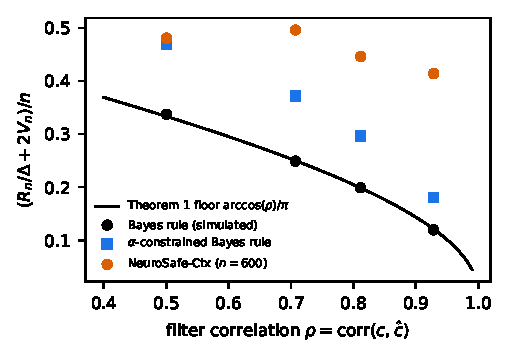
\includegraphics[width=0.6\linewidth]{figures/fig_floor.pdf}
\caption{\textbf{The floor of Corollary~1 and simulated policies} on the Gaussian threshold instance.}
\end{figure}
\end{document}
